\begin{question}
\noindent Triangle $A$ has vertices at $(-4, 3)$, $(-4, 5)$ and $(-1, 3)$.

\begin{center}
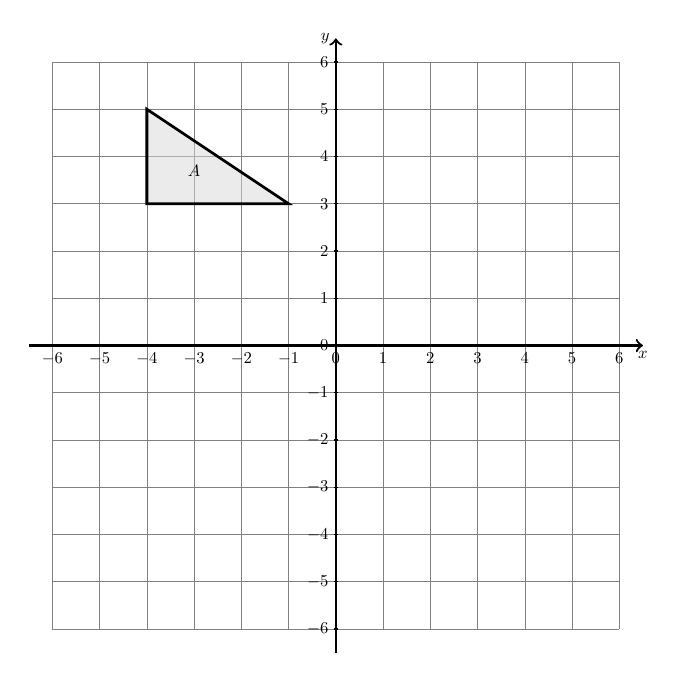
\begin{tikzpicture}[scale=0.6, transform shape]
    % Define colours
    \definecolor{borderColour}{HTML}{000000}
    \definecolor{fillColour}{HTML}{D8D8D8}

    % Define axis scale
    \def\axisLimit{6}

    % Draw grid
    \draw[step=1cm,gray,very thin] (-\axisLimit,-\axisLimit) grid (\axisLimit,\axisLimit);

    % Draw axes
    \draw[thick,->] (-\axisLimit-0.5,0) -- (\axisLimit+0.5,0) node[anchor=north] {$x$};
    \draw[thick,->] (0,-\axisLimit-0.5) -- (0,\axisLimit+0.5) node[anchor=east] {$y$};

    % Label x-axis and y-axis
    \foreach \x in {-\axisLimit,...,\axisLimit}
        \draw (\x cm,1pt) -- (\x cm,-1pt) node[anchor=north] {$\x$};
    \foreach \y in {-\axisLimit,...,\axisLimit}
        \draw (1pt,\y cm) -- (-1pt,\y cm) node[anchor=east] {$\y$};

    % Define coordinates for the vertices of triangle A
    \coordinate (P) at (-4,3);
    \coordinate (Q) at (-4,5);
    \coordinate (R) at (-1,3);

    % Draw triangle A
    \filldraw[fill=fillColour, draw=borderColour, line width=1pt, fill opacity=0.5] (P) -- (Q) -- (R) -- cycle;

    \node at (-3, 3.7) {$A$};

\end{tikzpicture}
\end{center}

\noindent Reflect triangle $A$ in the line $y = 1$.

Find the coordinates of the image of each vertex of triangle $A$.

\vspace{4cm}
\answerplain{2}
\end{question}
